\documentclass{beamer}

\PassOptionsToPackage{utf8}{inputenc}
    \usepackage{inputenc}

\usepackage{graphicx}

\usetheme{Boadilla}

\title{Essays in Computational Management Science}
\author{Marcelo Salhab Brogliato}
\institute{EBAPE / FGV}
\date{\today}

\setlength{\parskip}{\baselineskip}

\begin{document}

\begin{frame}
\titlepage
\end{frame}


\begin{frame}
\frametitle{Introduction}

Modern management and high technology interact in multiple, profound, ways. A whole new ecosystem seems to have emerged within computing and business.

The corporate biography of Tonny Martins, President of IBM Brasil, mentions his successes with blockchain, AI, and cognitive technology \emph{as an executive}, not as a research scientist or specialized engineer.

Professor Andrew Ng tells students at Stanford's Graduate School of Business that ``AI is the new electricity'', as his hyperbolic way to emphasize the potential transformational power of the technology.
\end{frame}

\begin{frame}
\frametitle{Introduction}

Both iPhone (and competitors) and Bitcoin (and competitors) have created giant platforms on top of which immense wealth has been created.

\end{frame}


\begin{frame}
\frametitle{Outline}
\begin{enumerate}[I]
\item Hathor: An alternative towards a scalable cryptocurrency
\item An invitation to Sparse Distributed Memory: from the theoretical model to the system dynamics
\item Diffusion and dismissal of innovation: forecasting the number of Facebook’s active users
\end{enumerate}
\end{frame}


\part{Hathor: An alternative towards a scalable cryptocurrency}
\begin{frame}
\frametitle{Hathor: An alternative towards a scalable cryptocurrency}

The problems: lack of scalability, centralization, and spam attacks.



\end{frame}


\begin{frame}
\frametitle{Cryptocurrency issues}

\begin{figure}
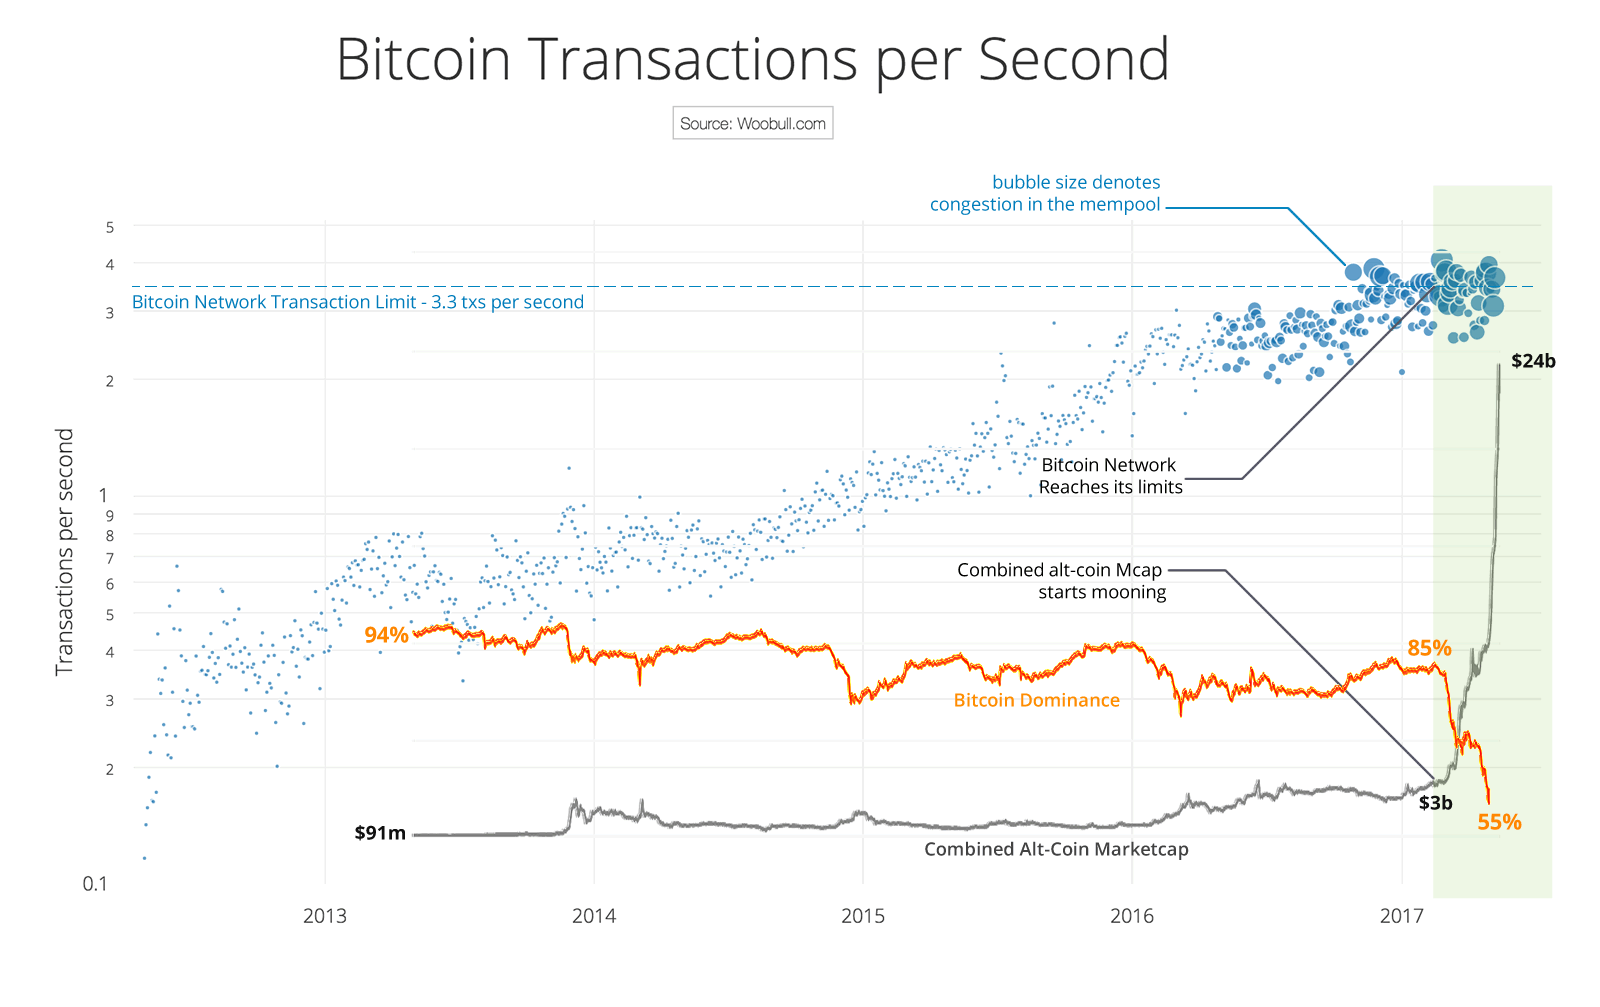
\includegraphics[width=\textwidth]{./images-defense/bitcoin-congestion.png}
\end{figure}

\end{frame}


\begin{frame}
\frametitle{Contributions}

The main contributions are:
\begin{enumerate}[i]
\item Mathematical analysis of Bitcoin
\item Proposal of Hathor
\item Analysis of Hathor
\end{enumerate}
\end{frame}


\begin{frame}
\frametitle{Bitcoin}

The primary problem for creating digital money is how to prevent double spending.

As the money is digital, and copies can be made \emph{ad nauseam}, what can prevent counterfeiting? What would prevent users from sending copies of the same money to two (or more) people?

The no central point of trust and predictable money supply together with a clever solution to the double-spending problem is what separates Bitcoin from the 30-year literature on e-cash.

\end{frame}


\begin{frame}
\frametitle{Blockchain (1)}

Each attempt to find a new block is equivalent to a random sample from a discrete uniform distribution in the interval $[0, 2^{256}-1]$. A new block is only found when the sample is less than a given number $A$.

The mining process is a sequence of failed attempts followed by a successful attempt. Let $X$ be the number of attempts until finding a new block. Then, $X$ follows a geometric distribution with probability $p = \frac{A}{2^{256}}$.

Let $H$ be the network hashpower, i.e., the number of attempts per second that the network is able to calculate. Thus, the time to find a new block (or the time between blocks) is $T = X/H$.

As $H$ changes over time, the given number $A$ is adjusted so that the network would find a block every $\eta$ seconds, which leads to $P(T \le t) = 1 - \left(1 - \frac{1}{\eta H} \right)^{tH}$.
\end{frame}


\begin{frame}
\frametitle{Bitcoin's hashpower history}
\begin{figure}
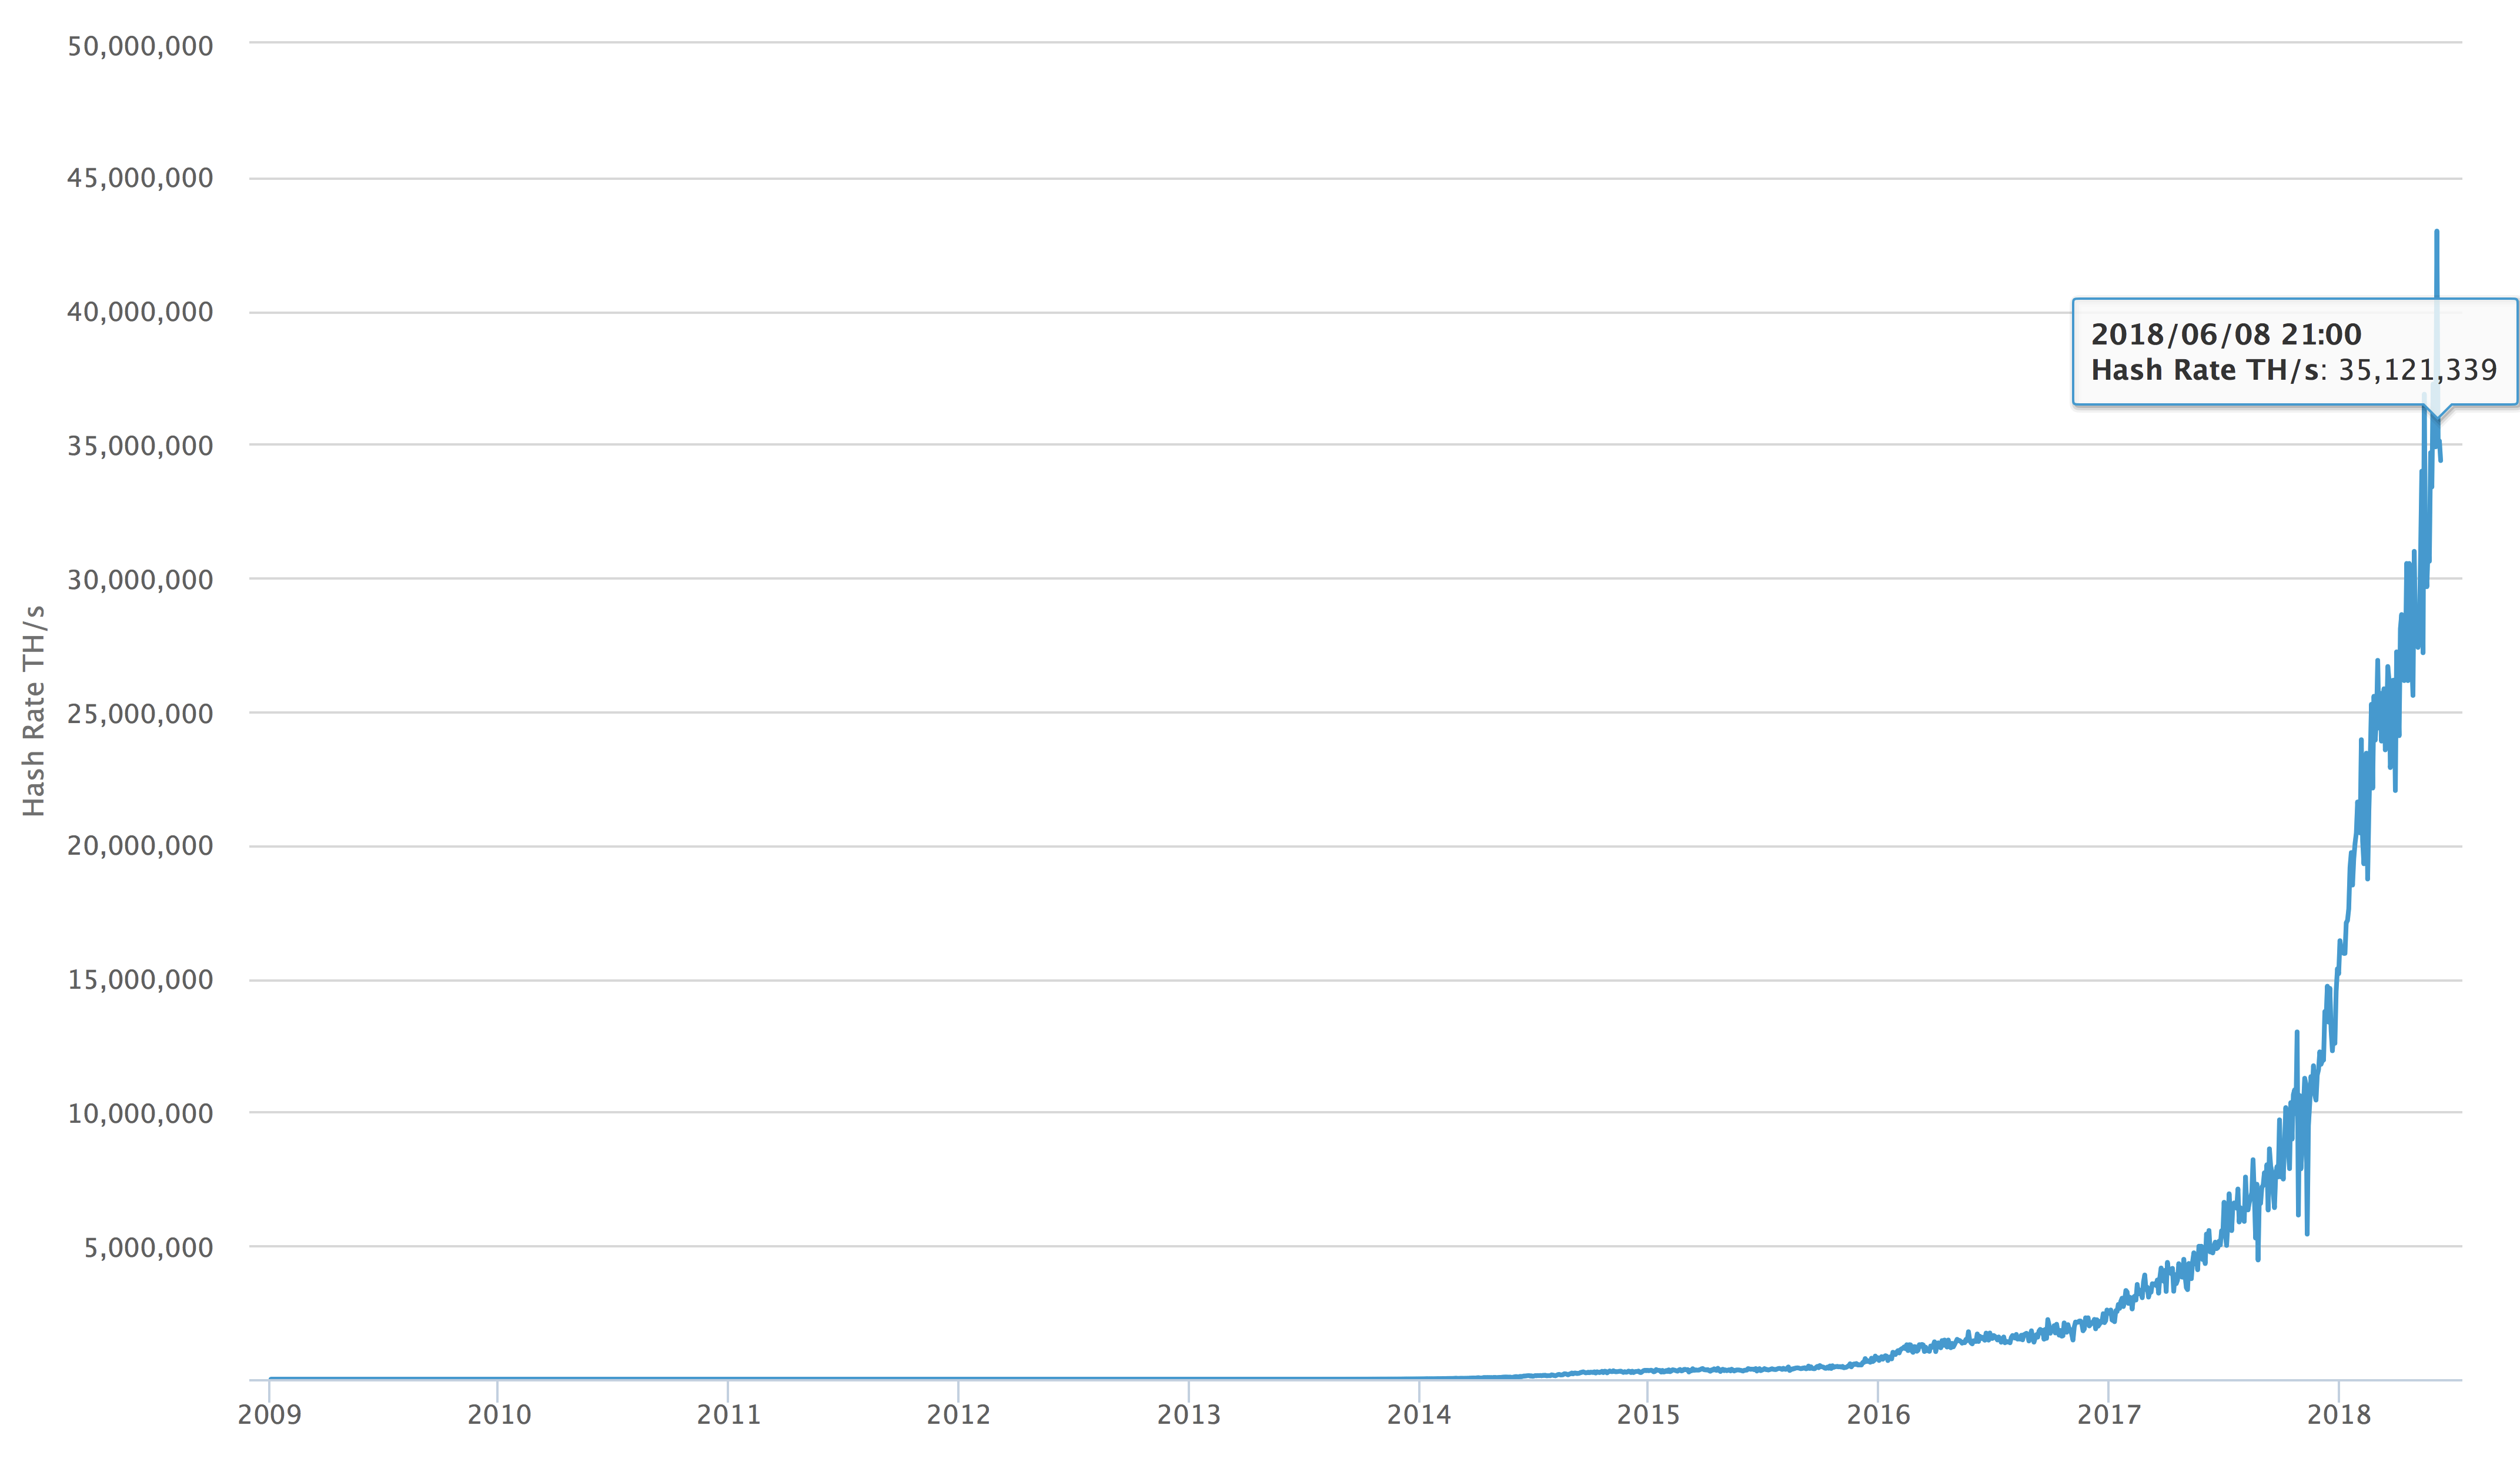
\includegraphics[width=\textwidth]{./images-defense/bitcoin-H-history.png}
\end{figure}
\end{frame}


\begin{frame}
\frametitle{Blockchain (2)}

\begin{theorem}
    For $H$ large enough, the time between blocks may be approximated by an exponential distribution, i.e., $P(T \le t) = 1 - e^{t/\eta}$.
\end{theorem}

\begin{theorem}
	The maximum absolute error when approximating the time between blocks by an exponential distribution is $e / H$.
\end{theorem}

So, for a maximum absolute error of $0.01 \% = 10^{-4}$, the network hashpower $H$ must be at least 26 kH/s.

For comparison, Bitcoin's hashpower is around 35,000,000 TH/s = 35,000,000,000,000,000 kH/s = $35 \cdot 10^{18} H/s$. In this case, the maximum absolute error is $7.7 \cdot 10^{-20} = 0.0000000000000000000776$.

\end{frame}


\begin{frame}
\frametitle{Blockchain (3)}

Let $Y_n = \sum_{i=1}^n T_i$ be the total time to find $n$ consecutive blocks. From probability literature, $Y_n$ follows an Erlang distribution.

\begin{figure}
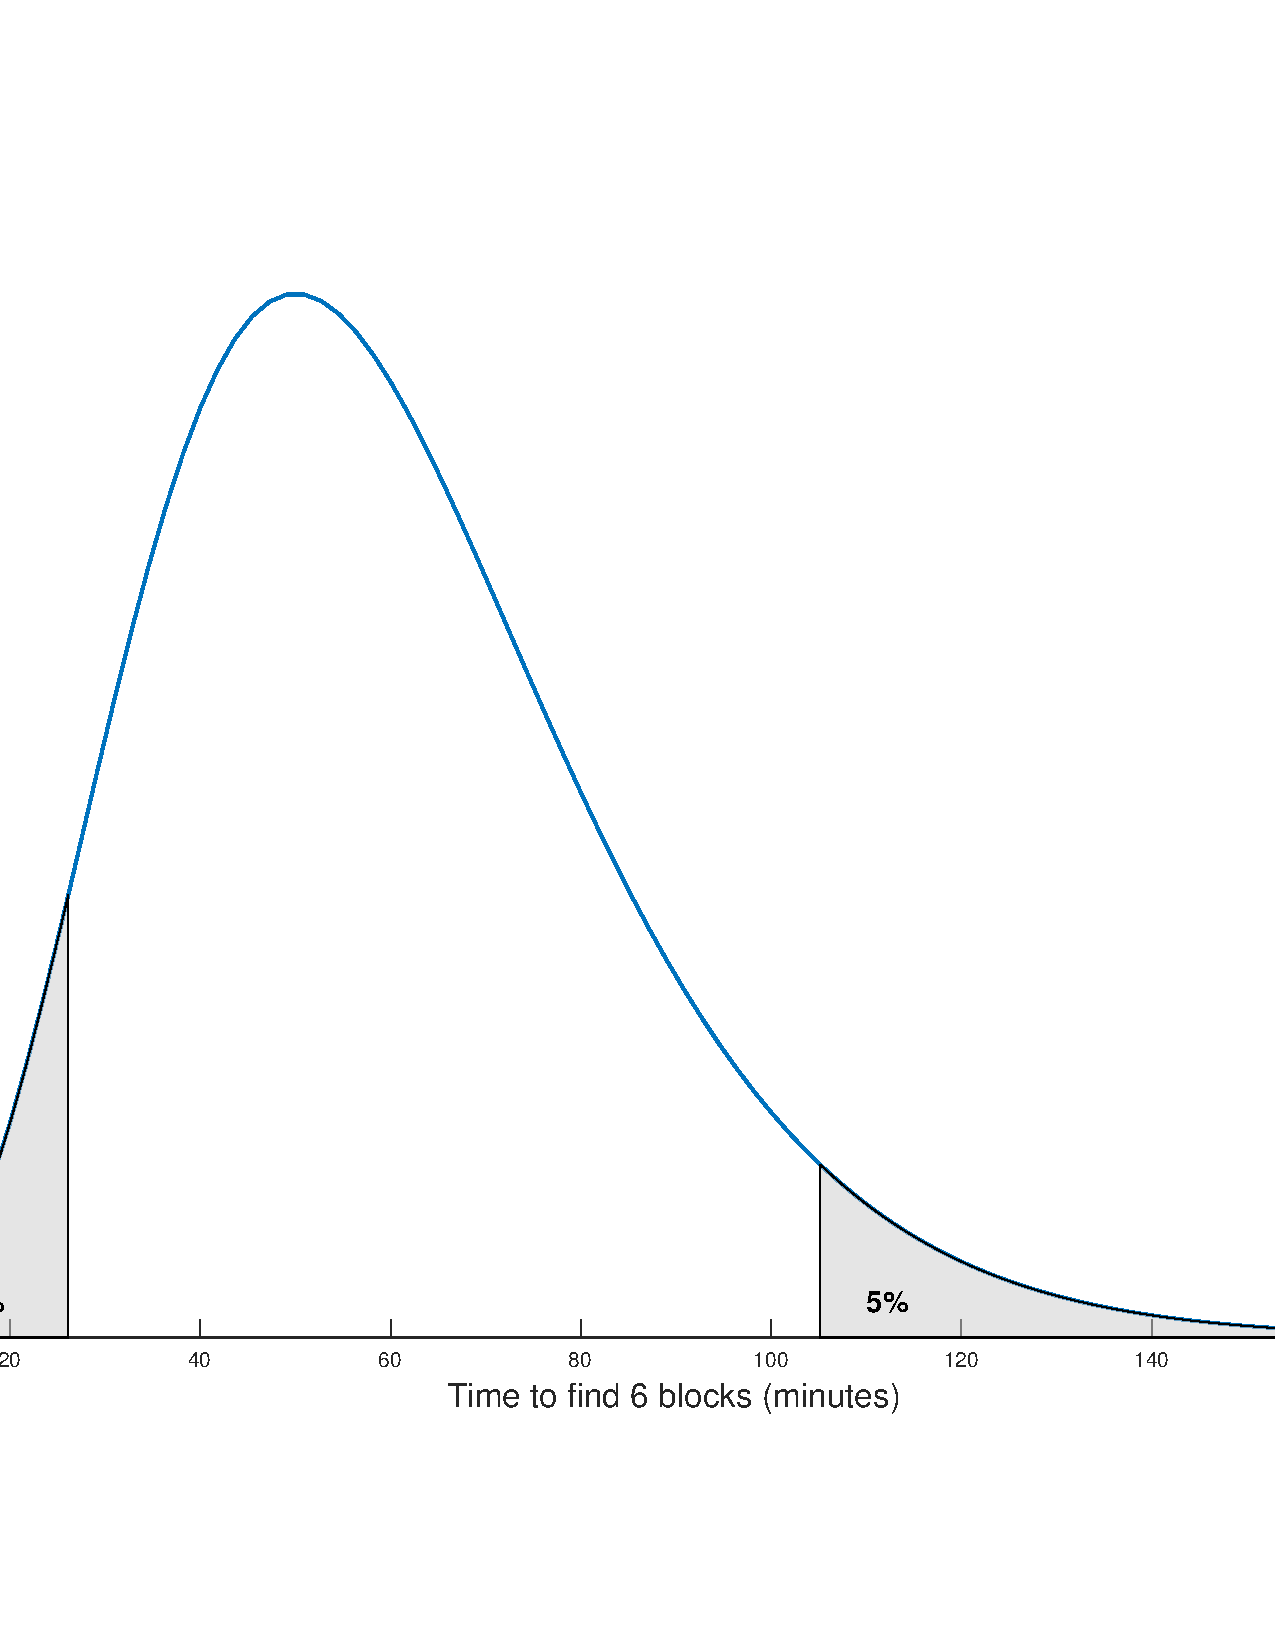
\includegraphics[width=0.7\textwidth]{./images01/time-6-blocks.pdf}
\caption{PDF of $Y_6$, i.e., probability of finding 6 consecutive blocks.}
\end{figure}

\end{frame}


\begin{frame}
\frametitle{Attack in the Bitcoin network}

\begin{theorem}
	Let $\beta$ be the percentage of the hashpower controlled by the attacker, and $\gamma$ the percentage of the hashpower without the attacker. Let $p = \frac{\gamma}{\beta + \gamma}$. Then,
$$
\mathbf{P}(\text{successful attack}) =
\begin{cases}
	1 - \sum_{s=0}^{k-1} \binom{k+s-1}{s} \left( (1-p)^s p^k - (1-p)^k p^s \right) \text{, $p \geq 0.5$} \\
	1 \text{, $\gamma < \beta$}.\\
\end{cases}
$$
\end{theorem}

For $k=6$, $p=0.9$, $\mathbf{P}(\text{successful attack}) = 0.0005914121600000266$.

For $k=6$, $p=0.7$, $\mathbf{P}(\text{successful attack}) = 0.15644958192000014$.

\end{frame}


\begin{frame}
\frametitle{Attack in the Bitcoin network}
\begin{figure}
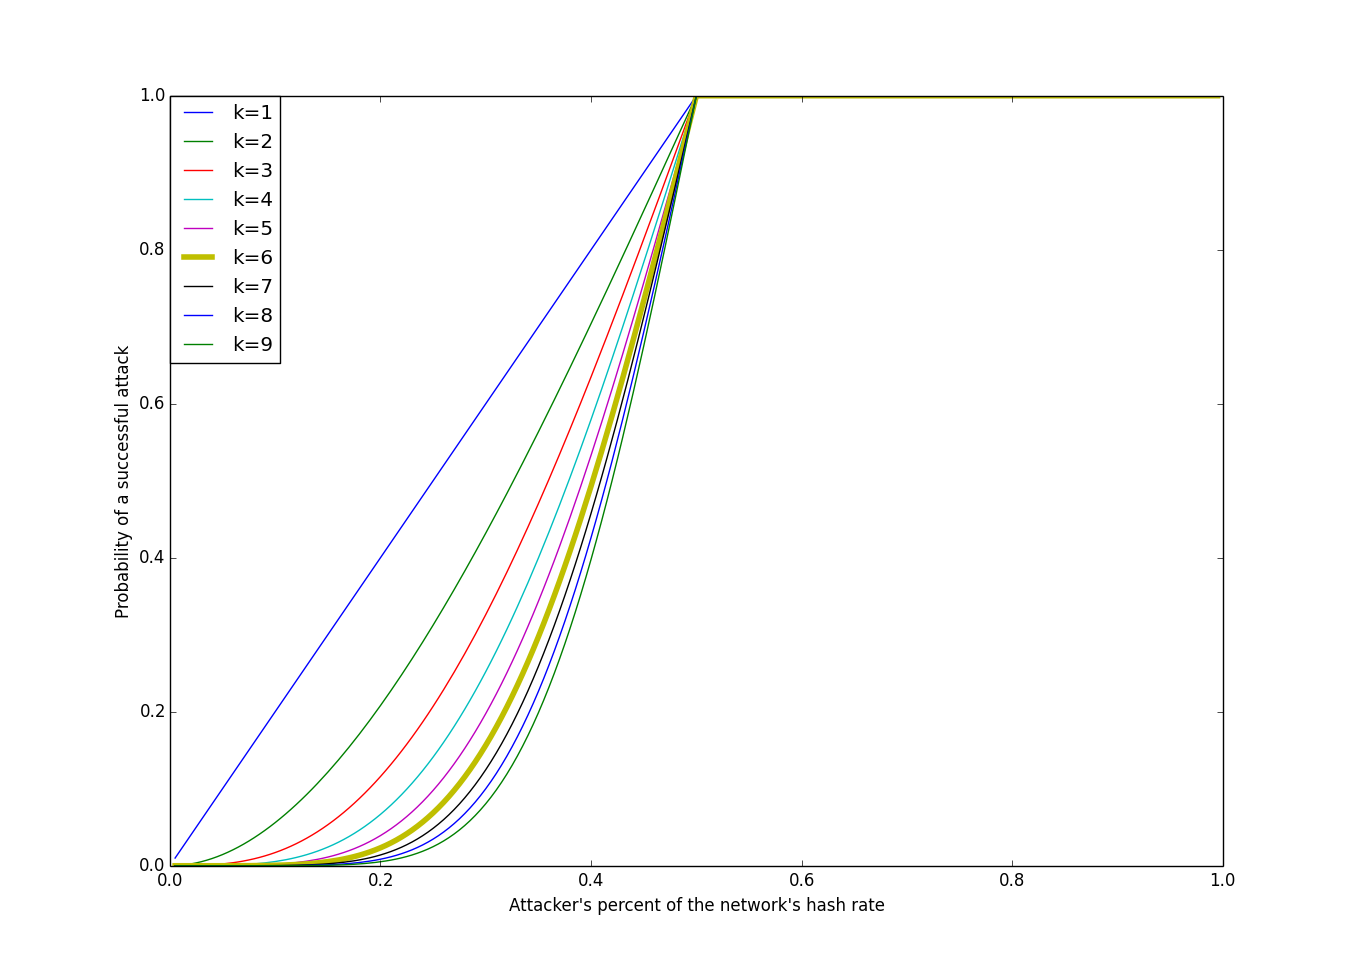
\includegraphics[width=0.75\textwidth]{./images01/fig-bitcoin-attack.png}
\caption{Probability of a successful attack according to the network's hash rate of the attacker ($\beta$).}
\end{figure}
\end{frame}



\part{An invitation to Sparse Distributed Memory: from the theoretical model to the system dynamics}
\begin{frame}
\frametitle{An invitation to Sparse Distributed Memory: from the theoretical model to the system dynamics}

The main contributions are:
\begin{enumerate}[i]
\item A validated, open-source, cross-platform framework
\item Identification and modeling of the autocorrelation in the counters
\item Noise filtering application
\item Classification application
\item Reinforcement learning application
\end{enumerate}
\end{frame}


\part{Diffusion and dismissal of innovation: forecasting the number of Facebook’s active users}
\begin{frame}
\frametitle{Diffusion and dismissal of innovation: forecasting the number of Facebook’s active users}

The main contributions are:
\begin{enumerate}[i]
\item Add a rejection parameter to the model
\item Estimate the parameters using only the number of active users
\item The possibility of reducing the number of active users (instead of only increase)
\end{enumerate}
\end{frame}

\begin{frame}
\frametitle{Conclusion}
\end{frame}


\end{document}
